\documentclass[10pt, t]{beamer}
\usetheme{metropolis}           % Use metropolis theme

\ifnotes
  \hypersetup{final}
  \usepackage{pgfpages}
  \setbeamertemplate{note page}[plain]
  \setbeameroption{show notes on second screen=right}
\fi

\usepackage{appendixnumberbeamer}
\usepackage{multirow}
\usepackage{verbatim}
\usepackage{solarized}            % use solarized themed listings
\usepackage{tikz}
\usetikzlibrary{decorations.pathreplacing}
\usepackage[scale=3]{ccicons}   % creative commons icons

\title{Parallel computing platforms}
\date{}
\author{Jeremy Iverson}
\institute{College of Saint Benedict \& Saint John's University}
\begin{document}
  \maketitle

  \begin{frame}{plan for the day}
    \begin{itemize}
      \item Naive Bayes assignment updates (40min + 5min break)
      \item parallel computer organization (40min + 5min break)
      \item classes of parallel computation (40min + 5min break)
      \item our first parallel algorithms (40min + 5min break)
    \end{itemize}
  \end{frame}

  \begin{frame}[standout]
    Naive Bayes in C
  \end{frame}

  \begin{frame}{parallel computer organization}
    \begin{itemize}
      \pause
      \item control mechanism
      \pause
      \item communication model
    \end{itemize}

    \note{
      \begin{itemize}
        \item in order to thinking about how we might solve problems using
          parallel computation, we need to understand what parallel capabilities
          our computing systems have.
        \item there are two fundamental questions we need to ask...
          \begin{itemize}
            \item control mechanism --- how are instructions executed in
              parallel
            \item communication model --- how do processing units communicate
          \end{itemize}
      \end{itemize}
    }
  \end{frame}

  \begin{frame}{flynn's taxonomy}
    \begin{itemize}
      \item based on the number of instruction streams and data streams
        available in the architecture
    \end{itemize}
    \vspace{1ex}
    \begin{columns}
      \begin{column}{.27\textwidth}
        \centering
        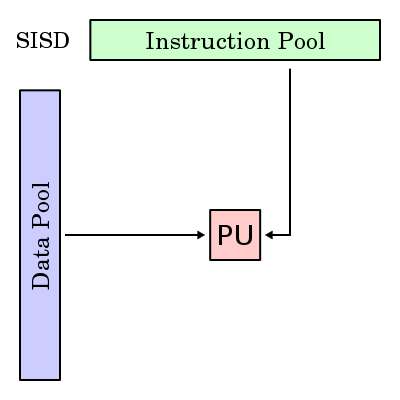
\includegraphics[width=\textwidth]{SISD.png}\\
        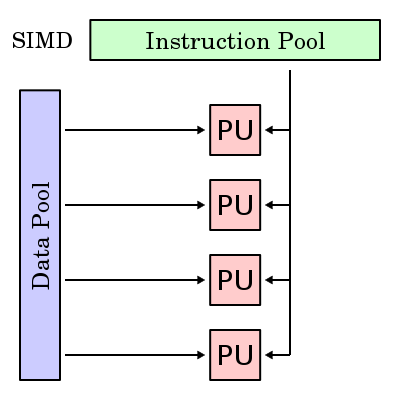
\includegraphics[width=\textwidth]{SIMD.png}
      \end{column}
      \begin{column}{.27\textwidth}
        \centering
        %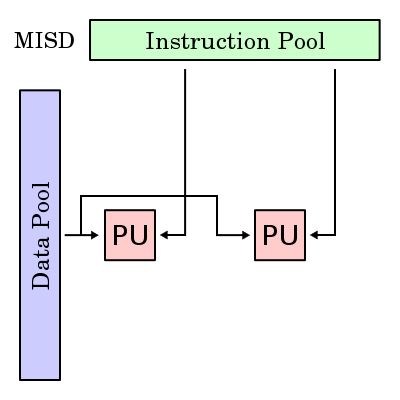
\includegraphics[width=\textwidth]{MISD.png}\\
        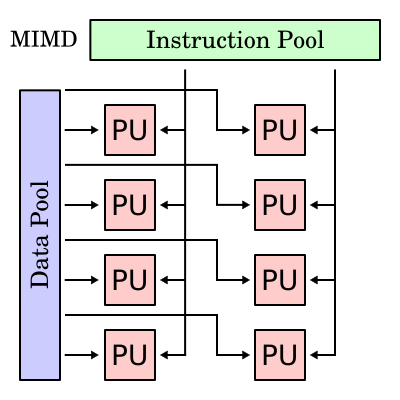
\includegraphics[width=\textwidth]{MIMD.png}
      \end{column}
    \end{columns}
    \hfill \tiny{\href{https://en.wikipedia.org/wiki/Flynn's\_taxonomy}{Flynn's~taxonomy}~by~Cburnett~/~\href{http://creativecommons.org/licenses/by-sa/3.0}{CC~BY~3.0}~/~presenting~the~four~together}

    \note{
      \begin{itemize}
        \item ask students to give examples of each
          \begin{itemize}
            \item SISD
              \begin{itemize}
                \item serial computer
              \end{itemize}
            \item SIMD
              \begin{itemize}
                \item gpu
                \item many modern cpus have simd extensions
              \end{itemize}
            \item MISD
              \begin{itemize}
                \item uncommon, but could be used for things like fault
                      tolerance
              \end{itemize}
            \item MIMD (in many cases, this is further divided into a category
              commonly known as SPMD, single program multiple data)
              \begin{itemize}
                \item most common type of parallel computer (multi-thread or
                  multi-node)
              \end{itemize}
          \end{itemize}
        \item which of these might be interesting to us, i.e., which might make
          good parallel systems?
      \end{itemize}
    }
  \end{frame}

  \begin{frame}[c]{simd}
    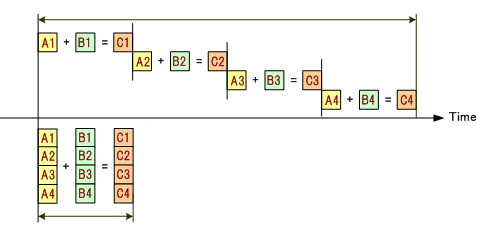
\includegraphics[width=\textwidth]{simd-execution.png}\\
    \hfill \tiny{\href{https://www.softek.co.jp/SPG/Pgi/TIPS/public/general/multicore-para.html}{SIMD}~/~cropped~from~original}

    \note{
      \begin{itemize}
        \item cuda / opencl are languages to express this type of parallelism,
          but we will not be studying them
        \item what sorts of problems might this be good for?
          \begin{itemize}
            \item matrix-oriented scientific computing
            \item media-oriented image and sound processors
          \end{itemize}
        \item simd is simpler and more energy efficient than mimd, why?
          \begin{itemize}
            \item only needs to fetch one instruction per ``cycle''
          \end{itemize}
        \item what would the mimd time line look like?
        \item so then what are the (dis)advantages of each of the
          classifications?
          \begin{itemize}
            \item simd works in lock stop, so does not require synchronization,
              which can make it easier to reason about
            \item mimd processing elements are autonomous, so can solve more
              complex problems
          \end{itemize}
      \end{itemize}
    }
  \end{frame}

  \begin{frame}{communication models}
    \begin{columns}
      \begin{column}{.48\textwidth}
        \begin{itemize}
          \item shared-address space
            %\begin{itemize}
            %  \item UMA / NUMA / ccNUMA
            %\end{itemize}
        \end{itemize}
      \end{column}
      \begin{column}{.48\textwidth}
        \begin{itemize}
          \item message-passing
        \end{itemize}
      \end{column}
    \end{columns}
    \vspace{3ex}
    \centering
    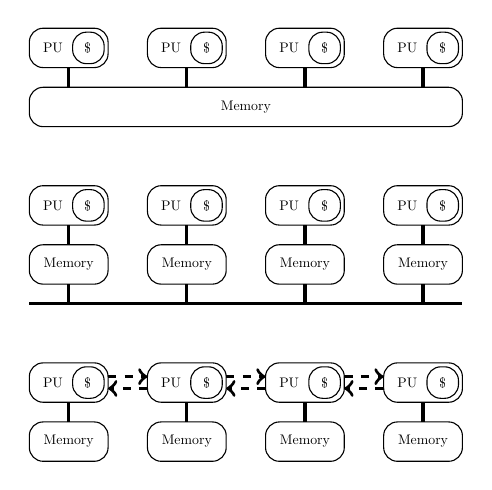
\begin{tikzpicture}[scale=.5,every node/.style={transform shape}]
      \foreach \x in {0,3,6,9}
      {
        \draw[very thick] ({\x+1},1) -- ({\x+1},1.5);
        \draw[rounded corners=5pt] (\x,1.5) rectangle ++(2,1);
        \node at ({\x+.6},2) {PU};
        \only<2>{\draw[rounded corners=5pt] ({\x+1.1},1.6) rectangle ++(.8,.8);}
        \only<2>{\node at ({\x+1.5},2) {\$};}
      }
      \draw[rounded corners=5pt] (0,0) rectangle ++(11,1);
      \node at (5.5,.5) {Memory};

      \foreach \x in {0,3,6,9}
      {
        \draw[rounded corners=5pt] (\x,-2.5) rectangle ++(2,1);
        \node at ({\x+.6},-2) {PU};
        \only<2>{\draw[rounded corners=5pt] ({\x+1.1},-2.4) rectangle ++(.8,.8);}
        \only<2>{\node at ({\x+1.5},-2) {\$};}
        \draw[very thick] ({\x+1},-3) -- ({\x+1},-2.5);
        \draw[rounded corners=5pt] (\x,-4) rectangle ++(2,1);
        \node at ({\x+1},-3.5) {Memory};
        \draw[very thick] ({\x+1},-4) -- ({\x+1},-4.5);
      }
      \draw[very thick] (0,-4.5) -- (11,-4.5);

      \foreach \x in {0,3,6,9}
      {
        \draw[rounded corners=5pt] (\x,-7) rectangle ++(2,1);
        \node at ({\x+.6},-6.5) {PU};
        \only<2>{\draw[rounded corners=5pt] ({\x+1.1},-6.9) rectangle ++(.8,.8);}
        \only<2>{\node at ({\x+1.5},-6.5) {\$};}
0
        \draw[very thick] ({\x+1},-7.5) -- ({\x+1},-7);
        \draw[rounded corners=5pt] (\x,-8.5) rectangle ++(2,1);
        \node at ({\x+1},-8) {Memory};
      }
      \foreach \u/\v in {2/3,5/6,8/9}
      {
        \draw[very thick,dashed,->] (\u,-6.35) -- (\v,-6.35);
        \draw[very thick,dashed,->] (\v,-6.65) -- (\u,-6.65);
      }
    \end{tikzpicture}

    \note{
      \begin{itemize}
        \item how do processing elements communicate with each other
          \begin{itemize}
            \item shared-address space
              \begin{itemize}
                \item everyone has access to everyone else's data
                \item communicate through shared memory
              \end{itemize}
            \item message-passing
              \begin{itemize}
                \item communicate through messages sent between PUs
                \item build on two basic operations, \emph{send} and
                  \emph{receive}
              \end{itemize}
          \end{itemize}
        \item why not just make everything uma?
        \item is there anything missing from this model?
          \begin{itemize}
            \item what is a cache for?
          \end{itemize}
        \item the existence of caches means that data can exist in multiple
          places
          \begin{itemize}
            \item a cache coherence protocol is required to ensure proper
              semantics and correct program execution
            \item have students think of a sequence of operations that would be
              incorrect without cache coherence
          \end{itemize}
      \end{itemize}
    }
  \end{frame}

  \begin{frame}{classes of parallel computation}
    \pause

    Imagine you are the head chef responsible for preparing a wedding banquet.
    The meal will have four courses: appetizer, salad, main course, and dessert.
    You have $P$ chefs at under your supervision.

    \pause

    How best to get the meal served to the guests as quickly as possible?

    \pause

    \begin{itemize}
      \item \only<4>{Each chef works on $N/P$ meals independently of the
        others.}\only<5>{\emph{data parallelism}}
      \item \only<4>{Each chef works on a different task related to the
        preparation of a meal, i.e., cutting carrots, cooking soup, icing cake,
        etc.}\only<5>{\emph{task parallelism}}
    \end{itemize}

    \note{
      \begin{itemize}
        \item With this understanding of parallel computation, we can think
          about how to formulate algorithms that expose some aspect of
          parallelism. Typically we will find ourselves in one of two
          situations, either:
          \begin{itemize}
            \item we have a bunch of different tasks to carry out, all of which
              can be done simultaneously
            \item we want to do the same task to a bunch of different inputs
          \end{itemize}
          it isn't always obvious which we have and sometimes the same problem
          can be expressed many ways.
      \end{itemize}

      \begin{itemize}
        \item Is this an example of SIMD or MIMD, neither or both? Why?
      \end{itemize}
    }
  \end{frame}

  \begin{frame}[fragile]{\texttt{y := a*x + y}}
    \begin{codeblock}
    void
    saxpy(size_t const n,
          float  const a,
          float  const * const x,
          float        * const y)
    {
      for (size_t i = 0; i < n; i++) {
        y[i] = a * x[i] + y[i];
      }
    }
    \end{codeblock}
  \end{frame}

  \begin{frame}[fragile]{reduction}
    \begin{codeblock}
    float
    min(size_t const n,
        float * const x,
    {
      /* x[0] will always contain the current
       * minimum */
      for (size_t i = 0; i < n; i++) {
        if (x[i] < x[0]) {
          x[0] = x[i];
        }
      }
      return x[0];
    }
    \end{codeblock}
  \end{frame}

  \begin{frame}[fragile]{reduction cont'd}
    \begin{codeblock}
    float
    min(size_t const n,
        float * const x,
    {
      for (size_t i = 1; i < n; i *= 2) {
        /* x[j] will always contain the current
         * minimum in interval [j,j+2i)*/
        for (size_t j = 0; j < n; j += 2 * i) {
          if (x[j + i] < x[j]) {
            x[j] = x[j + i];
          }
        }
      }
      return x[0];
    }
    \end{codeblock}
  \end{frame}

  \begin{frame}[fragile]{sorting}
    \begin{verbatim}
      count = array of k+1 zeros
      for x in input do
          count[x] += 1

      total = 0
      for i in 0, 1, ... k do
          counti = count[i]
          count[i] = total
          total += counti

      for x in input do
          output[count[x]] = x
          count[x] += 1

      return output
    \end{verbatim}
  \end{frame}

  \appendix

  \begin{frame}[c]
    \begin{center}\ccbysa\end{center}

    except where otherwise noted, this worked is licensed under
    \href{http://creativecommons.org/licenses/by-sa/4.0/}{creative commons
    attribution-sharealike 4.0 international license}
  \end{frame}
\end{document}
